\chapter{Background}
\label{chapter:background}
This thesis is based on several kinds of researches: auto-tuning, evolutionary algorithms, and software optimization. In this chapter we summarize the important aspects and details of approaches and optimization techniques, used within the thesis.  

\section{Multi-Quality Auto-Tuning~(MQuAT)}

Multi-Quality Auto-Tuning (MQuAT) – is an approach to self-adaptive software, which provides design and operation principles for software systems that automatically provide the best possible utility to the user while producing the least possible cost.
It is based on the design-time part, which represents a new development method for self-optimizing systems and runtime parts, which concerns operation principles, namely,  novel techniques to runtime self-optimization~\cite{gotz13}.
MQuAT allows software developers to build and run software systems, which are automatically adjusted to provide the optimal user utility for the minimal cost. Such systems are comprised of multiple variants differing in their non-functional behavior and can analyze the reasons for the trade-offs between the respective non-functional properties (NFPs).  A key characteristic of MQuAT is the use of Quality of Service contracts to cover the inter-dependencies between NFPs,  the distinction between hard- and software, and the use of behavioral models to simulate complex non-functional behavior like \textit{energy consumption}.
In this thesis, MQuAT is used as a software environment that provides an optimization problem.


\section{MQuAT Problem}
\label{sec:MQuATProblem}

MQuAT problem was presented in ~\cite{gotz18}, and could be presented as two problems:

\begin{itemize}
	\item \textbf{Resource allocation} in which the mapping of software component implementation to hardware resource leads to the least cost
	\item \textbf{Variant selection}, which provides the best utility by selecting better software implementations.
\end{itemize} 

The problem description uses the JastAdd framework\cite{ekman07} based on specified grammar~\cite{gotz2018JastAdd}. Aa a result, it gives a possibility of using reference attribute grammars~(RAGs)\cite{hedin2000} that adds computations in model nodes.

To solve this problem a new generic metamodel was presented. Both problems are interrelated by user requests specifying minimum requirements on the provided non-functional properties (i.e., minimum utility) while searching for a selection and mapping both to maximize utility and minimize costs. Correctness denotes that only solutions that \textit{do not violate} the user's minimum requirements are considered \textbf{valid}.

The problem to be solved is selecting variants of software components and mapping them based on user requests to suitable hardware resources.


The MQuAT problem could be described as a metamodel~(see Figure~\ref{fig:mquatmodel}) which consists of:
\paragraph{Hardware metamodel,}which consists of hierarchically structured resource types and resources as instances of these types. So the hardware model composes static resource types and runtime resource instances knowledge. Certain types of resources can run the software, i.e., they are valid targets for software implementation mapping. The container attribute is used to mark such types. Figure~\ref{fig:HWmodel} depicted Hardware metamodel.
\todo{just a formatting note: shouldn't the fig. captions be centered?}
\begin{figure}
	\centering
	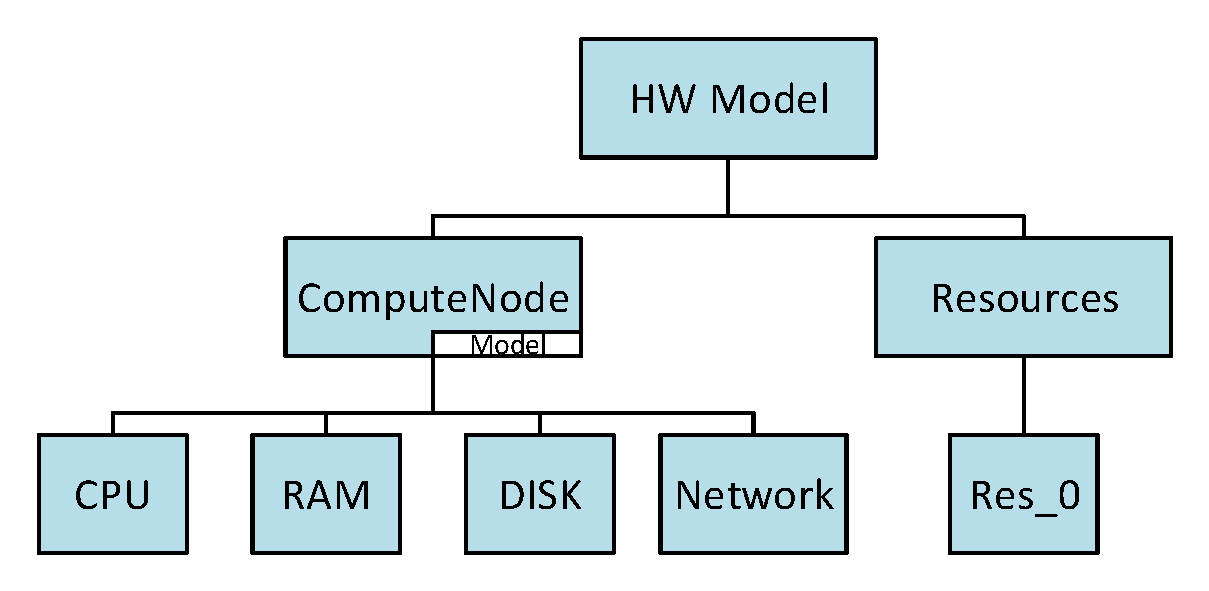
\includegraphics[width=0.8\textwidth]{images/HWModel.pdf}
	\caption[Hardware meta-model]{Hardware meta-model}
	\label{fig:HWmodel}
\end{figure}


In addition, a set of properties further characterizes resource types. Resources specify then concrete values for these properties. As an example, the resource type RAM could be defined with a property amount of memory and marked as a container.

\paragraph{Software metamodel} showed on Figure~\ref{fig:SWModel}. Its main element, called component, provides some functionality, required by the user.
Each component could have different implementations that provide this functionality, requiring additional components or resources to complete their work. 

\begin{figure}
	\centering
	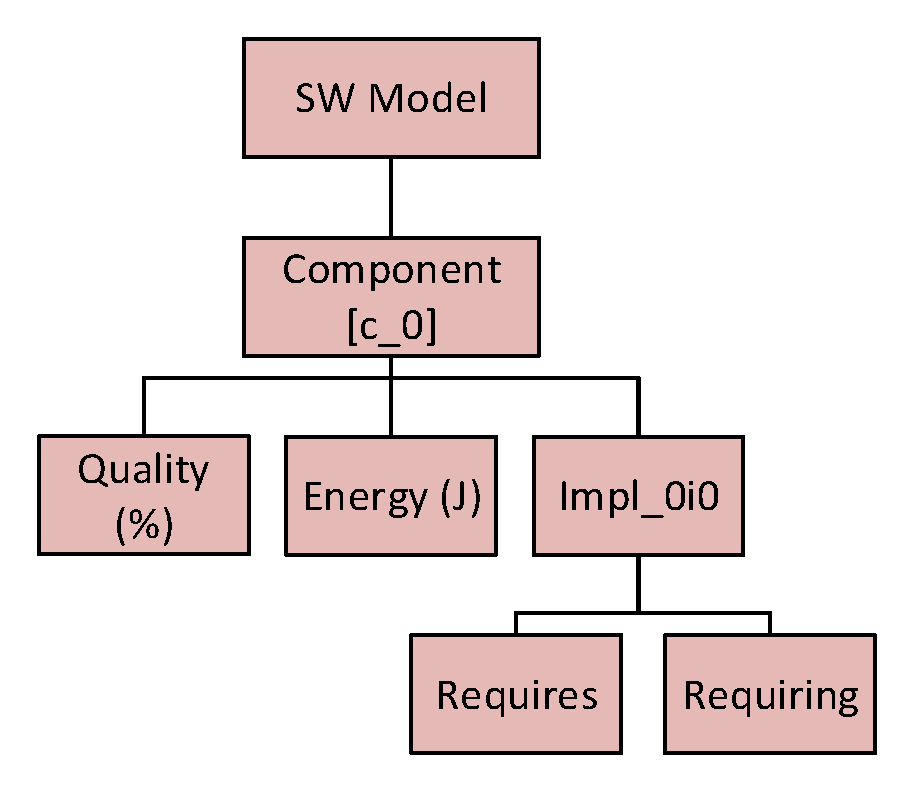
\includegraphics[width=0.5\textwidth]{images/SWModel.pdf}
	\caption[Software meta-model]{Software meta-model}
	\label{fig:SWModel}
\end{figure}

\paragraph{The Objective} specifies how to calculate a solution's objective value, i.e., for which value(s) the problem should be optimized. For example, minimize the energy consumption.

\paragraph{The Request} represents a user's specified functionality that should be executed with its parameters and requirements.  The request contains the functional requirements by referencing a target software component and limitations on non-functional requirements (e.g., quality).\\


\begin{figure}
	\centering
	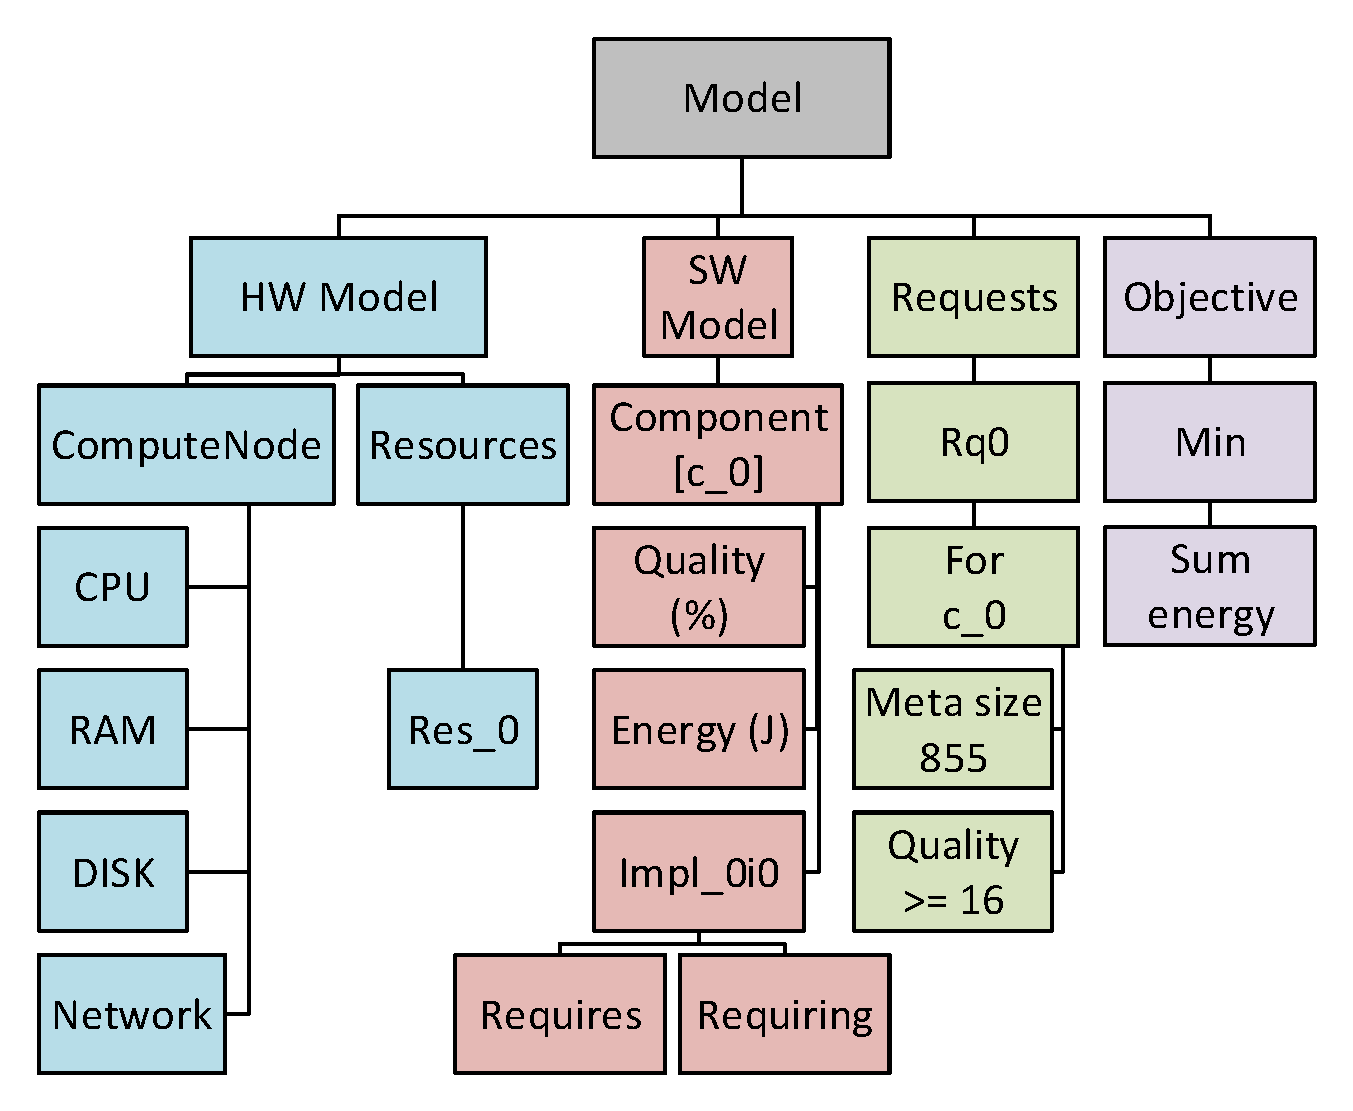
\includegraphics[width=0.8\textwidth]{images/MQuATModel.pdf}
	\caption[MQuAT problem model]{MQuAT problem model}
	\label{fig:mquatmodel}
\end{figure}


Due to the complexity of the MQuAT problem, some constraints grouped in Architectural, Request, and Negotiation constraints groups:

\begin{itemize}
	\item \textbf{Architectural constraints} ensure that each request is fulfilled, selecting exactly one implementation per component and deploying no more than one implementation on one resource.
	\item \textbf{Request constraints} ensure components are selected for each request so as to provide the requested non-functional properties.
	\item \textbf{Negotiation constraints} ensure non-functional requirements are met depending on the implementation.
\end{itemize}

There are additional constraints due to synthetic problem generation:

\begin{itemize}
	\item Structures for the software and hardware components are fixed to ensure comparability;
	\item \texttt{computeNode} that represents a regular computer hardware consist of one or more CPUs, RAM memory, disk, and a networking interface;
	\item Software model has a simple tree structure;
	\item Each software component could have 2 sub-components, or do not depend on sub-components. It means that each node of the tree structure has 2 sub-nodes, or it is a leaf of the tree.
\end{itemize}

Each MQuAT Problem is characterized by four parameters:

\begin{itemize}
	\item \textbf{Software variants} - the number of implementations for each software component,
	\item \textbf{Number of requests} - the number of requests to run software components, that described by user, 
	\item \textbf{Component tree depth} - the depth of the software tree that describes the dependency of software component that user requested,
	\item \textbf{Resources ratio} - this parameter describes the number of available hardware resources. The number of HW resources calculated as the multiplication of the number of nodes of the component tree by the number of requests and multiplied by the resource ratio.
\end{itemize}

\section{Solution of the MQuAT Problem}

The Solution is computed by the MQuAT Solver. There are many Solvers:

\begin{itemize}
	\item \textbf{Simple Solver}, which goes step by step from one solution candidate to another, enumerating solution candidates.
	\item \textbf{ILP Solver}, which generates Integer Linear Programming~(ILP) Problem from the MQuAT Problem and solves it.
	\item \textbf{Random Solver} - tries random solution candidates.
	\item \textbf{Simulated Annealing~(SA) Solver} - based on the Simulated Annealing meta-heuristic~\cite{pukhkaiev19}.
	\item \textbf{Genetic Solver} - uses a Evolution Algorithm to solve the problem.
\end{itemize}

In this thesis, we focus on Genetic Solver in detail in the next sections. The solution of the MQuAT Problem could be represented as a tree structure. An example of the Solution shown in Figure ~\ref{fig:SolutionModel}. It contains a list of assignments. Each assignment selects one implementation of the required component and maps it on the resources~\cite{gotz18}.


\begin{figure}
	\centering
	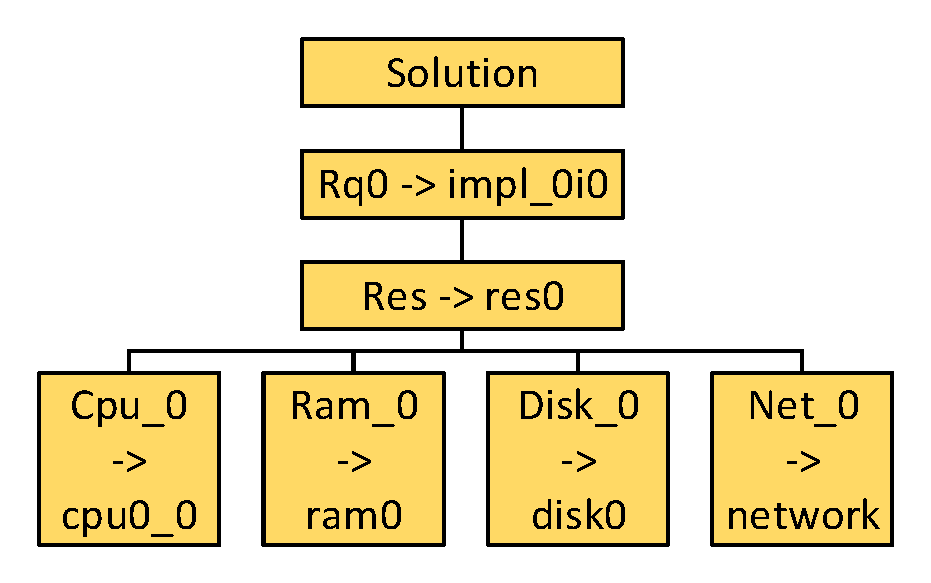
\includegraphics[width=0.5\textwidth]{images/MQuATSolutionModel.pdf}
	\caption[MQuAT solution model]{MQuAT solution model}
	\label{fig:SolutionModel}
\end{figure}


The Solution is valid if for each user request following requirements fulfilled:
\begin{enumerate}
	\item an implementation is deployed for the target component;
	\item an implementation is deployed for each required component;
	\item all necessary (non-functional) property clauses (including request constraints) are met;
	\item at most one implementation for each resource is deployed.
\end{enumerate}

The Solution is optimal if the Solution is valid, and no other solution has a better objective value~\cite{gotz18}.

\section{Evolutionary Algorithms}
\label{sec:GeneticAlgorithm}

Evolutionary algorithms (EA) are a subset of evolutionary computation and belong to the set of modern heuristics-based search methods.~\cite{vikhar16}
This domain contains different variants, such as:
\paragraph{Genetic algorithm~(GA)} - is the most widely known type of EA\cite{eiben03}. The research~\cite{deJong75} presented the description of the simple GA that represents a solution as a binary string. GA uses proportional selection, and a low probability of mutation. It has a fixed flow. The entire population changes in each generation. Currently, more preferable to use the rank-based selection, one-point crossover changed to the alternatives. And most important, that developers use not a binary representation that increases an understanding of the problem that GA is solving.
\paragraph{Evolution strategy~(ES)} - that works with vectors representation of a solution. New offspring is generated by adding random values to the elements in the vector. Use self-adaptation for own parameters. ES self-adapt the mutation step sizes.
\paragraph{Evolutionary programming~(EP)} - was developed with the aim to get artificial intelligence~\cite{eiben03}. It has the same representation as ES, but do not use the recombination. The selector algorithm selects parents from the union of the population and new offspring.
\paragraph{Genetic programming~(GP)} - use as a representation of solutions tree-shaped structures. Recombination works by sub-tree exchanging. A particular difference is in the workflow. A GP performs either a crossover or a mutation, and a GA performs two operations in sequence.

The main difference between them is a solution representation that called the \textbf{Genotype} or the \textbf{chromosome}. Each genotype consist of \textbf{genes} which represents the minimal element of the solution. A genotype in a form that could be evaluated is \textbf{Phenotype}. A set of genotypes~(chromosomes) is a population.

\begin{figure}
	\centering
	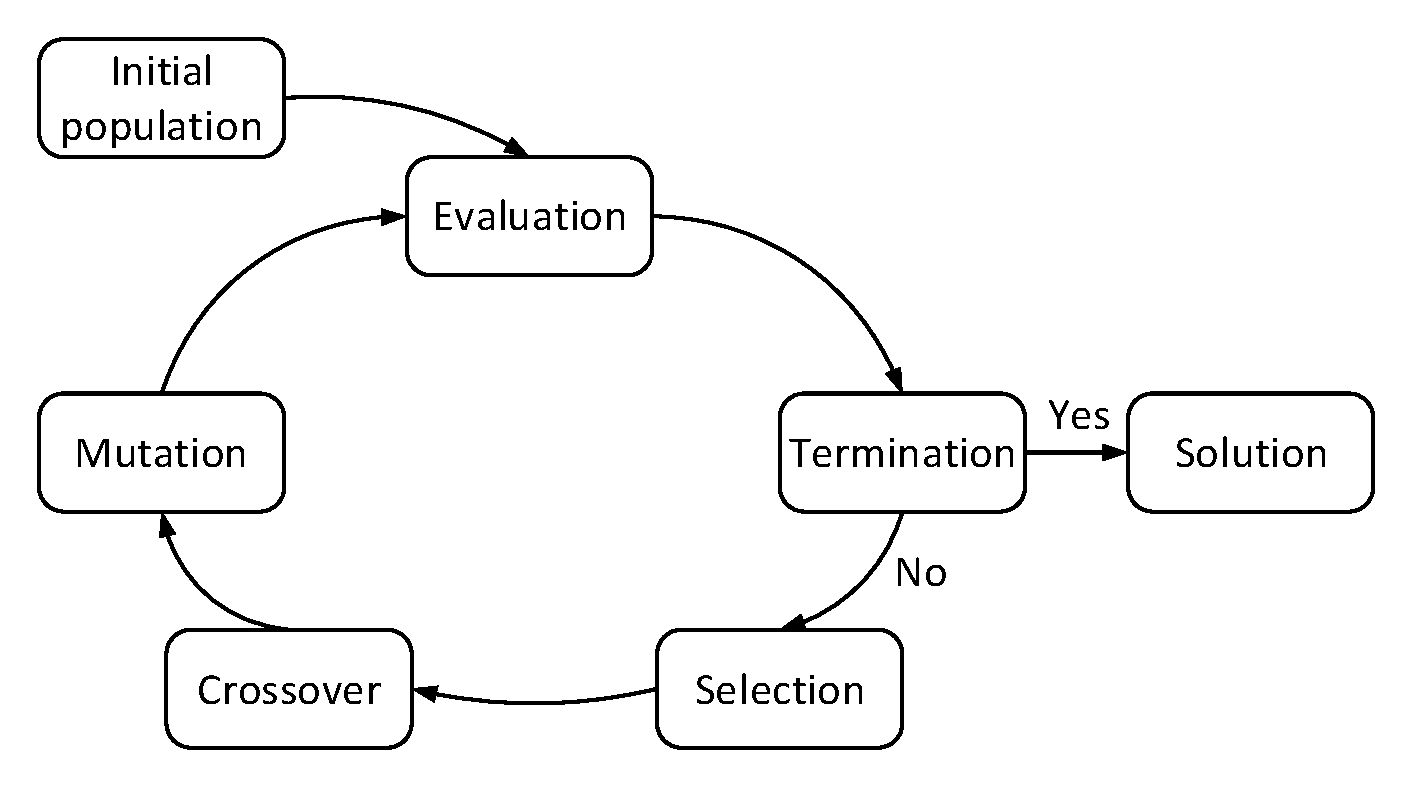
\includegraphics[width=0.8\textwidth]{images/GeneticLoop.pdf}
	\caption[The main loop of the evolutionary algorithm]{The main loop of the evolutionary algorithm}
	\label{fig:GeneticLoop}
\end{figure}

Any EA is based on different components and operators that construct it flow.
Figure~\ref{fig:GeneticLoop} shows the main principle of EA. It looks like a loop with iteratively repeated steps.
The first step is the creation of an initial population - a set of randomly created genotypes;
The second step is Evaluation. Calculate the fitness or objective function of the current population.
If the solution is founded and all requirements for the termination are fulfilled, then we get the final solution. Otherwise, select the best candidates to create a new generation.
In step 4, using Recombination and Mutation on selected candidates, GA creates a new generation of the population. And after that, evaluate it.

\subsection{Selector}\label{sec:GeneticAlgorithm:Selector}

The Selector is one of the most important components of the EA. It selects \textit{\textbf{mu}} chromosomes from the population, that are used to create new \textit{\textbf{lambda}} chromosomes. This process is called \textit{Selection algorithm}. There are many different Selection algorithms.


\paragraph{NSGA-II~(Non-dominated sorting based genetic algorithm)~\cite{deb2000}} - is a multi-objective selection algorithm. It searching for non-dominated solutions. Figure~\ref{fig:nsga2} demonstrates how it works. There is a population \texorpdfstring{R\textsubscript{t}}{R t} that consist of two sets. First set is a parent population. It is marked as \texorpdfstring{P\textsubscript{t}}{P t}. The second set is new offspring and denoted as \texorpdfstring{Q\textsubscript{t}}{Q t}. Combined population \texorpdfstring{R\textsubscript{t}}{R t} is sorted using non-dominated sorting. After that it generates a Pareto front. After sorting, selector selects the new population \texorpdfstring{P\textsubscript{t+1}}{P t+1} of size represented as a parameter by binary tournament selection and use it for the next round of reproduction.

\begin{figure}
	\centering
	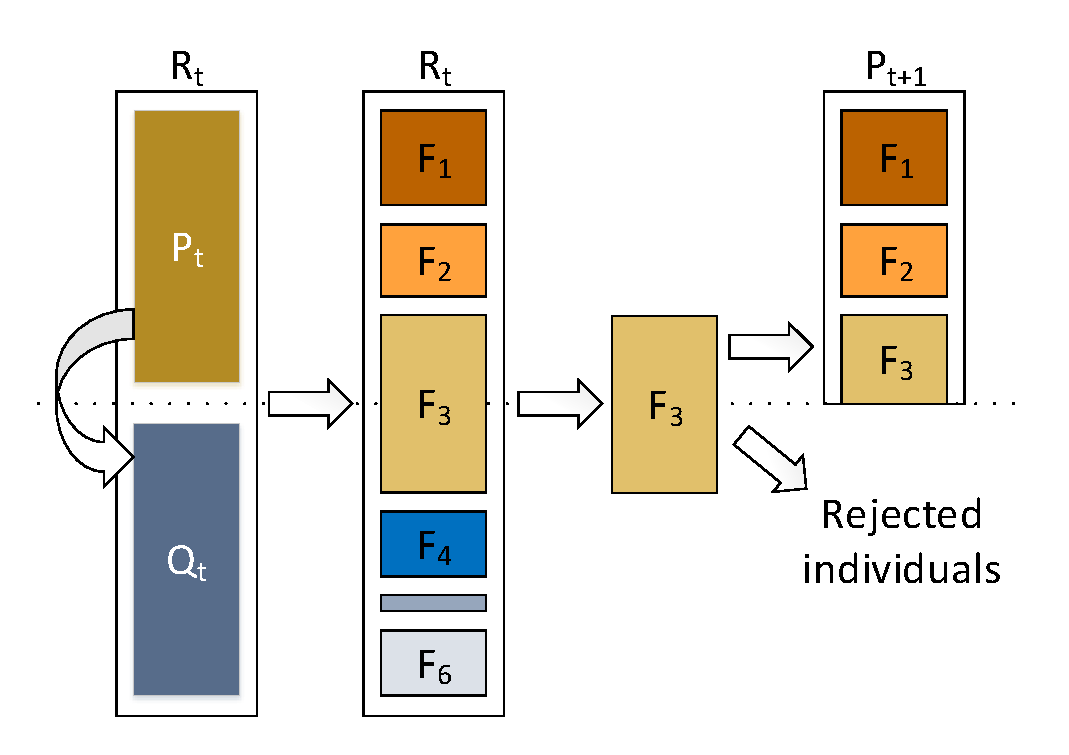
\includegraphics[width=0.75\textwidth]{images/nsga2.pdf}
	\caption[NSGA-II selection algorithm]{NSGA-II selection algorithm}
	\label{fig:nsga2}
\end{figure}

\paragraph{SPEA2~(Strength Pareto Evolutionary Algorithm)~\cite{zitzler01}} - a multi-objective selection algorithm, that used to find the Pareto optimal solution for multi-objective problems\cite{zhihuan2010}. Figure~\ref{fig:spea2} demonstrate how it works.
There are two sets. First one is a current population that denoted as \texorpdfstring{R\textsubscript{t}}{R t}. The second is an archive set. It is marked as \texorpdfstring{A\textsubscript{t}}{A t}. SPEA2 takes the union of all solutions in \texorpdfstring{R\textsubscript{t}}{R t} and in \texorpdfstring{A\textsubscript{t}}{A t}. The union set is marked as \texorpdfstring{U\textsubscript{t}}{U t}. After that it compares the size of \texorpdfstring{U\textsubscript{t}}{U t} and archive size. If \texorpdfstring{U\textsubscript{t}}{U t} is grater than archive size then SPEA2 reduce the union population. If \texorpdfstring{U\textsubscript{t}}{U t} is less  size then SPEA2 extend the population from the dominated solutions. After that, it selects best non-dominated solutions that used in next iteration.

\begin{figure}
	\centering
	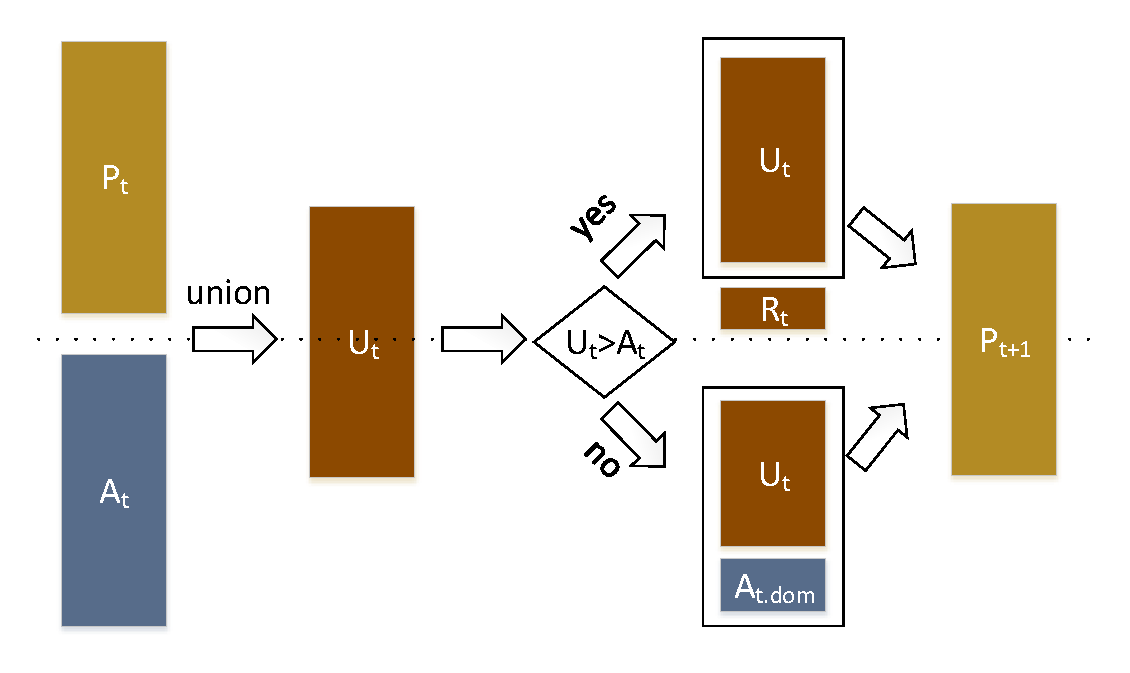
\includegraphics[width=0.9\textwidth]{images/spea2Selector.pdf}
	\caption[SPEA2 selection algorithm]{SPEA2 selection algorithm}
	\label{fig:spea2}
\end{figure}

\paragraph{NSGA3~\cite{deb14}} - it extends NSGA-II to using reference points to handle multi-objective problems, and its usage on one- or two-objective problems is discouraged.
\paragraph{SPEA3} - presented in~\cite{rudzinski15}. It is a generalization of SPEA2 that consists of the exchange of the selection procedure that aims to determine the non-dominated solutions with a high spread and balanced distribution. As described in researches, it works well with two- and three-objective problems. \\

In this thesis, we focus on a Selection algorithm only as a parameter of a genetic algorithm and use NSGA-II and SPEA2 due to software constraints of the used framework. 

\subsection{Crossover}\label{sec:GeneticAlgorithmCrossover}

Crossover is an operator of the EA that allows the recombination of two genotypes by swapping some genes between them.
In general, the crossover has several parameters such as

\begin{itemize}
	\item Crossover rate - parameter that describes the probability of two chromosomes to exchange their genes.
	\item Crossover point - the point in which the exchange could be done.
\end{itemize}

The principle of the crossover is next.
Firstly, select the crossover point. For example, a chromosome could be described as a vector of bits. Then the crossover point is the start index of bits, which were replaced by another chromosome.
Secondly, it swaps genes between chromosomes.

\begin{figure}
	\centering
	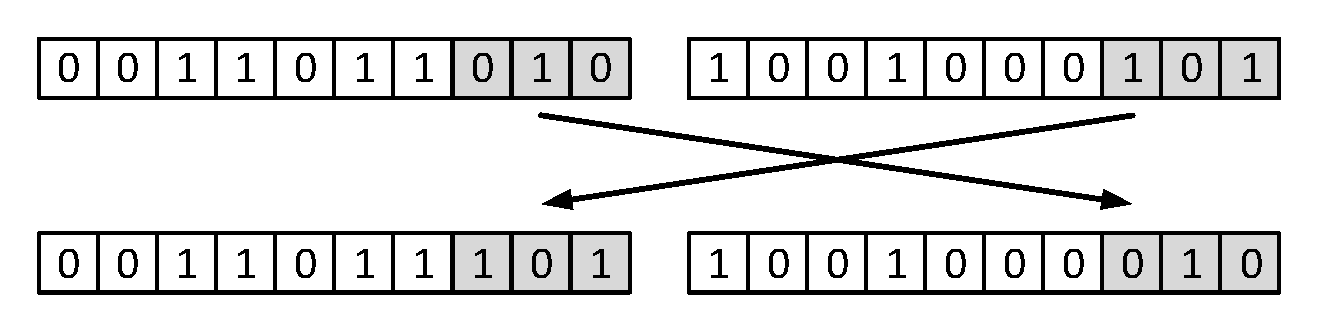
\includegraphics[width=0.6\textwidth]{images/crossoverVector.pdf}
	\caption[Example of the Crossover]{Example of the Crossover between chromosomes that described as a vector of bits}
	\label{fig:crossoverVector}
\end{figure}

\subsection{Mutation}\label{sec:GeneticAlgorithmMutation}

The mutation is an operator of the EA that changes a single gene in a chromosome. Similarly to the crossover, a mutation has parameter \texttt{Mutation rate}. It describes the probability of mutation.

To perform a mutation on chromosome it is needed to:

\begin{enumerate}
	\item Randomly select gene which mutates
	\item Change selected gene to another.
\end{enumerate}

\begin{figure}
	\centering
	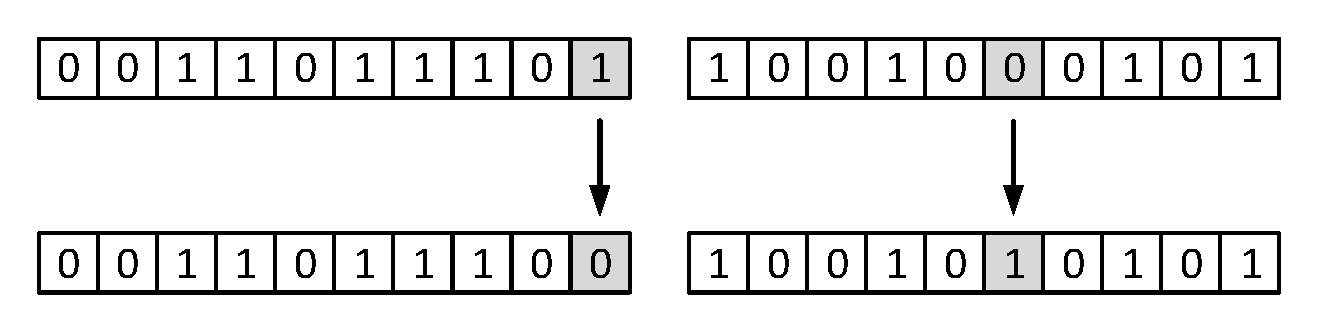
\includegraphics[width=0.6\textwidth]{images/mutationVector.pdf}
	\caption[Example of the Mutation]{Example of the Mutation in a chromosome that described as a vector of bits}
	\label{fig:MutationVector}
\end{figure}

Figure~\ref{fig:MutationVector} presented a simple mutation on the chromosome that is described as a vector of bits.




\section{Genetic Solver}\label{sec:GeneticSolver}
The Genetic Solver was created to solve the MQuAT Problem. It was developed by Jamal Ahmad in~\cite{ahmad18}. And further improved by Johannes Mey.

This Solver is based on Opt4J framework~\footnote{http://opt4j.sourceforge.net}. It is an open-source framework that gives the opportunity to implement an EA for custom optimization problem.

Several classes created to solve the MQuAT Problem using EA. There are:

\begin{enumerate}
	\item Genotype - is a custom developed genotype that could represent tree shaped structure of the solution.
	\item Crossover operator - describes the algorithm of the crossover for custom developed genotype.
	\item Mutation operator - describes the algorithm of the mutation for custom developed genotype.
	\item Creator is needed to create a random genotype for the initial population.
	In the genetic solver Creator create the genotype by creating a random solution model and transform it into a Tree Shape Genotype structure.
	\item Decoder is needed to perform decoding the tree shape genotype into phenotype. The phenotype, in this case, is a Solution Model of MQuAT.
	\item Evaluator that calculates the objective functions of the Solution. In the case of genetic solver, the Evaluator calculates two objectives: 
	
	\begin{itemize}
		\item Validity errors - the number of violated contracts
		\item Energy value - the energy consumption
	\end{itemize}
	
\end{enumerate}

\subsection{Tree Shape Genotype}

Because of the problem model of MQuAT, which requires mapping of implementations to resources, in genetic solver was created Tree Shape Genotype~\cite{ahmad18}.
The example of this genotype shown on Figure~\ref{fig:TreeShapeGenotypeExample}

\begin{figure}
	\centering
	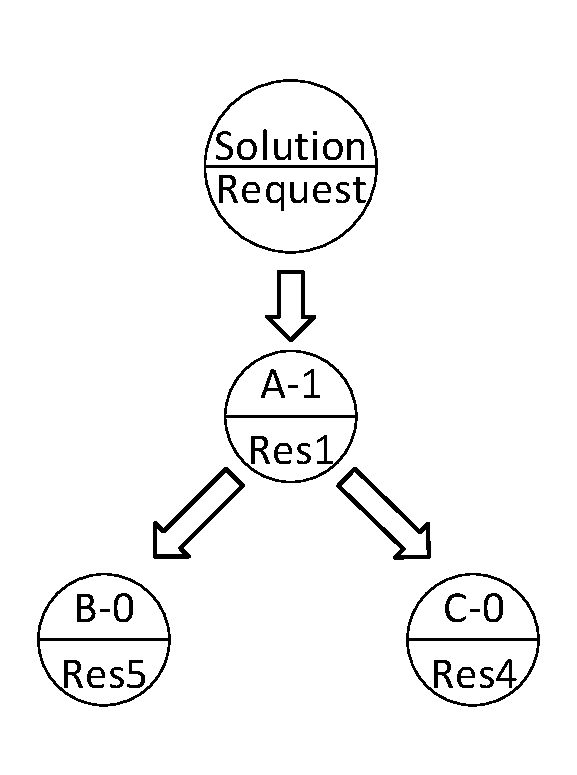
\includegraphics[width=0.6\textwidth]{images/TreeShapeGenotypeExample.pdf}
	\caption[Example of the Tree Shape Genotype]{Example of the Tree Shape Genotype}
	\label{fig:TreeShapeGenotypeExample}
\end{figure}

The first node in this genotype contains the input request. The second node represents the mapping of the user component. In this node, Impl A-1 is selected rather than Impl A-0 of the user component. As shown in Figure~\ref{fig:TreeShapeGenotypeExample}, this implementation is mapped to Hardware-Resources1. Moreover, Impl A-1 also requires software components B and C that have only one Impl B-0 and Impl C-0 implementation and are mapped to Hardware-Resource5 and Hardware-Resource4, respectively.

\subsection{Crossover Operator}
\label{sec:GeneticSolverCrossover}

This operator performs a crossover between two Tree Shaped Genotypes. The process starts on the root of both trees. Crossover operator compares if the implementation and mapped resources of both nodes are the same. If not the same, then with probability described as a parameter \texttt{CrossoverProbability}, it swaps the implementations, resources, and lower substructure of the tree. It swaps the subtree in order to maintain consistency. If comparison says that nodes are identical, then it performs the crossover process for each child node. Such a recursive algorithm gives a possibility to perform the crossover on a few points of the Tree Shape Genotype, as it showed in Figure~\ref{CrossoverPoints}. Crossover points have a gray color.

\begin{figure}
	\centering
	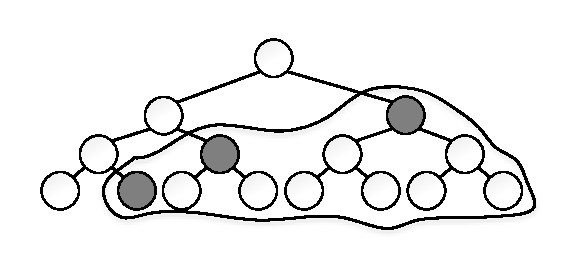
\includegraphics[width=0.5\textwidth]{images/CrossoverPoints.pdf}
	\caption[Crossover Points]{Crossover Points}
	\label{fig:CrossoverPoints}
\end{figure}

Figure~\ref{fig:GeneticSolverCrossover} depicted the crossover between two genotypes. Each genotype has 3 nodes. The Crossover starts on the root nodes. These nodes have the same implementation and resources. As a result, crossover recursively goes down to children. As shown, the first child of both genotypes has different implementation and resource, and crossover swap them with the probability \texttt{CrossoverProbability}. After that crossover operator performs a comparison for the second child.


\begin{figure}
	\centering
	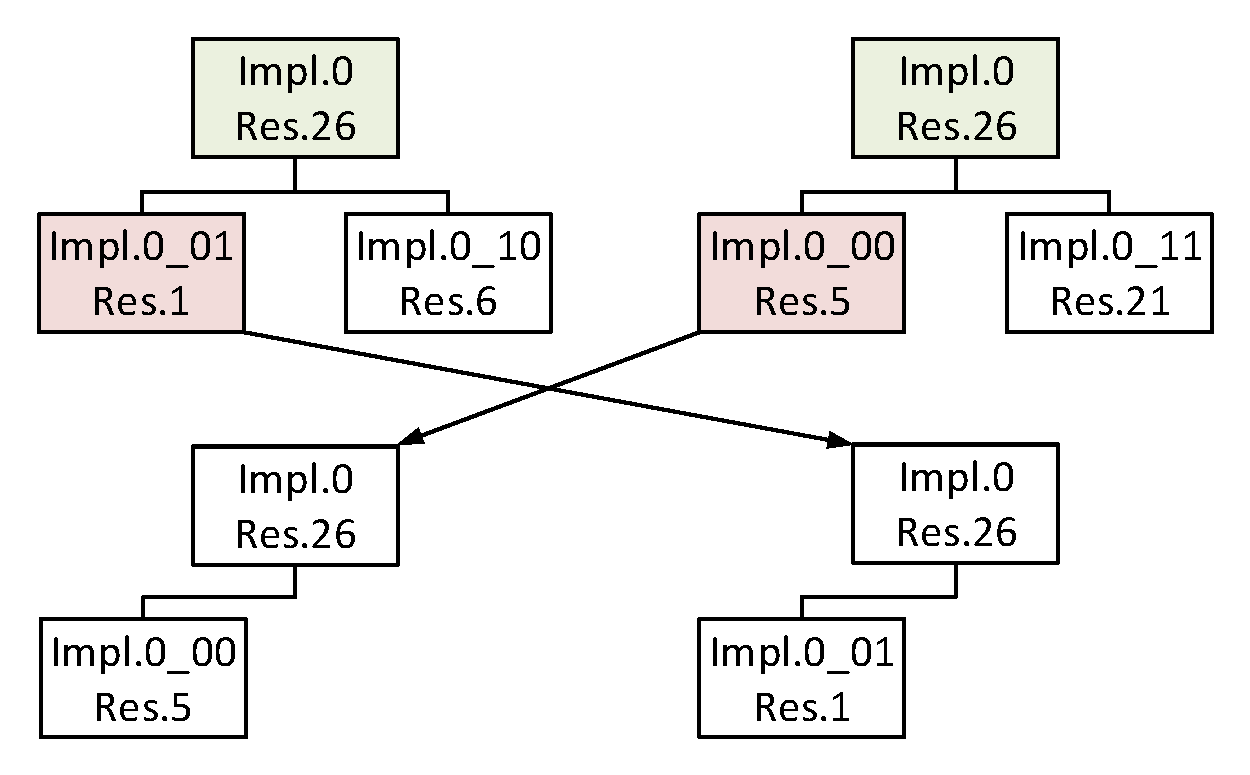
\includegraphics[width=0.6\textwidth]{images/GeneticSolverCrossover.pdf}
	\caption[Crossover in Tree Shape Genotype]{Example of crossover between two Tree Shape Genotypes}
	\label{fig:GeneticSolverCrossover}
\end{figure}



\subsection{Mutation Operator}
\label{sec:GeneticSolverMutation}
Mutation operation is used to randomly change the node(s) of the Tree Shaped Genotype.
The mutation occurs for one random request. With some probability that described by parameter \texttt{MutationRate}, it mutates the root node. If a mutation operator mutates the top node of the tree, there is a probability of the resource mutation. This probability described with parameter \texttt{ResourceMutationProbability}. Or it will mutate the implementation of the top node. And change the lower structure for consistency. If mutation occurs not in the root of the genotype, then the process recursively goes down to children.  Figure~\ref{fig:GeneticSolverMutation} depicts the mutation process in which mutation was performed on the resource 
in the root node.

\begin{figure}
	\centering
	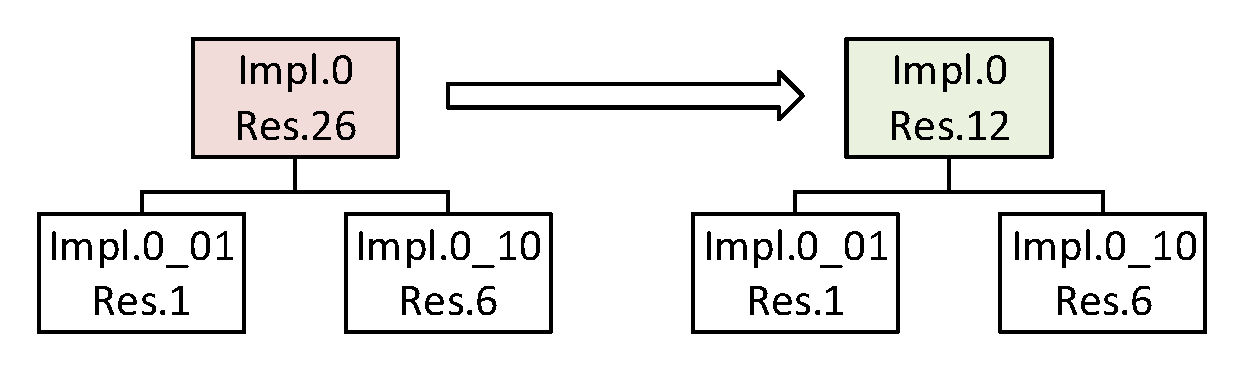
\includegraphics[width=0.6\textwidth]{images/GeneticSolverMutation.pdf}
	\caption[Mutation in Tree Shape Genotype]{Example of mutation between two Tree Shape Genotypes}
	\label{fig:GeneticSolverMutation}
\end{figure}

\section{Parameter Tuning Strategies for Evolutionary Algorithms}\label{sec:Parameter Tuning Strategies}

There are many parameters used by EA to solve the optimization problem. And we believe that "good" parameter values could improve EA. There are different approaches exist. 
The first approach of the parameter tuning adheres to select the values of parameters by some conventions, ad-hoc choices, or by experimental comparison on a limited scale. Such a tuning strategy based on assumptions about user-preferences and the influence of parameter values~\cite{eiben03,eiben11}. For example, the developer tries to tune 4 parameters and 10 values for each of them.
The drawbacks of this approach are:
\begin{itemize}
	\item Parameters could depend on each other. As a result, they can not be optimized one by one.
	\item Trying all possible combinations is difficult and requires a huge amount of time. To test 4 parameters with 10 possible values, need more than 1 million runs. If we run it at least 3 times to achieve some level of accuracy, then we need to run EA more than 3 million times. If a single run of the EA needs 1 minute, then parameter tuning will be finished after \textbf{5 years}. 
	\item If parameters are numerical or continuous. The optimal value may not be in the tested values.
\end{itemize}

We can conclude that parameter tuning without automation and without the understanding of the process is not working. Tuning an algorithm requires a lot of computer power,
while some people argue that this is a waste of time~\cite{smit2009comparing}.

As a result, 2 different approaches to choosing parameters were described: Parameter tuning and parameter control~\cite{smit2012parameter,eiben03}.
\textit{Parameter tuning} finds optimized values of parameters before the run. So all parameters are fixed and do not change during the run. However, \textit{parameter control} sets the values of parameters while EA is running. So the parameter was initially given, but during the run, the parameter value is changing. 

\subsection{Parameter Control}
As mentioned before, parameter control could adjust EA parameters on-the-fly. A run of the EA is a dynamic process, and using static parameters could be optimal only for some state, problem, or stage of EA. 
The simplest example of such technic is Rechenberg's 1/5 success rule~\cite{rechenberg1973evolutionsstrategie}. It describes how to change mutation parameters using information about the number of successful mutations. Commonly such features based on the developed feedback mechanism that contains information about the search process.

Parameter control consist of 3 categories:
\begin{itemize}
	\item \textbf{Deterministic parameter control} - parameter value adjusted by the deterministic rule without any feedback. 
	\item \textbf{Adaptive parameter control} - it uses some feedback from the EA as input for parameter changes. The value of the parameter may depend on the quality of the solution. Parameter changing is not a part of EA that solves the optimization problem.
	\item \textbf{Self-adaptive parameter control} - parameters are part of the chromosome. As a result, better chromosomes lead to better parameter values.
\end{itemize}
In this thesis, we focused on parameter tuning of EA, but we understand that parameter control is a very important approach that could significantly improve the results.

\subsection{Parameter Tuning}\label{sec:parameterTuning}
All parameter tuning methods could be divided into 2 categories: model-free and model-based~\cite{hutter2010}.
The first category trying to find "good" parameter values that give the best result of EA to be tuned. Examples of such tuners are F-Race~\cite{birattari2010f} and ParamILS~\cite{hutter2009paramils}.

\paragraph{F-Race} is a racing method that was adapted to fine-tune stochastic search methods~\cite{montero2012state}. To compare sets of parameter values, it uses Friedman two-way analysis\cite{theodorsson87} of variance by ranks. This method does not require any additional hypothesis about the search space. It works until complete all search space, or when a defined number of configuration is analyzed. The F-Race has the following parameters:
\begin{itemize}
	\item initial number of runs without calibrations,
	\item the confidence level,
	\item the max budget,
	\item the ranges of all parameters.
\end{itemize}

\paragraph{ParamILS} - The Parameter Iterated Local Search is performing parameter tuning as an iterated local search algorithm. It starts the optimization process with default parameter values and goes further. It moves from the default set to the neighborhood. On each iteration, it takes a few sets of parameter values and performs a local search to find out the best configuration. The ParamILS has the following parameters:
\begin{itemize}
	\item the number of configurations for the first iteration,
	\item the number of tested configuration per iteration,
	\item a restart probability,
	\item the max budget.
\end{itemize}


The second type is a more complex solution. Such tuners build a model that predicts the results of EA for given parameter values. As a result, different models or heuristics are used to reduce the number of tests. The model builds based on data about parameters and results that parameters give. The examples of model-based tuners are: Sequential Parameter Optimization~(SPO)~\cite{bartz2004analysis}, Bonesa~\cite{smit2012parameter, bartz2005sequential} REVAC~\cite{nannen2007efficient} and BRISE~\cite{pukhkaiev2016, pukhkaiev19}.

\paragraph{REVAC} - the Relevance Estimation and Value Calibration of EA. Works as an estimation of distribution algorithm~\cite{pelikan2002, montero2012state}. It represents each parameter as a set of values. The REVAC starts for each parameter the search process that uses the uniform distribution of values. It also performs a transformation of parameter sets to reduce the range of values and perform a predefined number of runs. This tuner appropriate for ordered parameters. The REVAC has parameters:
\begin{itemize}
	\item the number of elements in a set,
	\item step sizes of set modifications,
	\item the max number of iterations.
\end{itemize} 

\paragraph{BRISE} - the software product line (SPL) for parameter tuning. The work concept consists of a combination of local search and model prediction. It starts with the selection algorithm, which selects a new set of parameters. After that, the model rebuilds on each iteration and predicts the best parameter values. The BRISE is a more generic approach and used not only for EA. It has many parameters that describe its components. \\

The experimental comparison in~\cite{smit2009comparing} shows that no matter what tuner is used, it gives a better EA than relying on intuition and the usual parameter setting conventions.

In conclusion, there are many tuners that could help get optimized parameter values for EA. They have different methodologies to tune parameters such as models or selectors to select parameter values from several places of the search space. This overview shows that we could use all types of tuners. 

Due to the fact that a genetic solver requires a big amount of time to solve the task, we decide to use one of the model-based tuners. We will use a model-based tuner. And BRISE is more generic than others. 

\section{BRISE}\label{sec:BRISE}

BRISE is a software product line (SPL) for parameter tuning~\cite{pukhkaiev19}.3
This SPL has two conceptual parts:

\begin{itemize}
	\item Static part describes the main flow of parameter tuning, task management, and reporting.
	\item Configurable parts should be configured for each experiment.
\end{itemize}

\begin{figure}
	\centering
	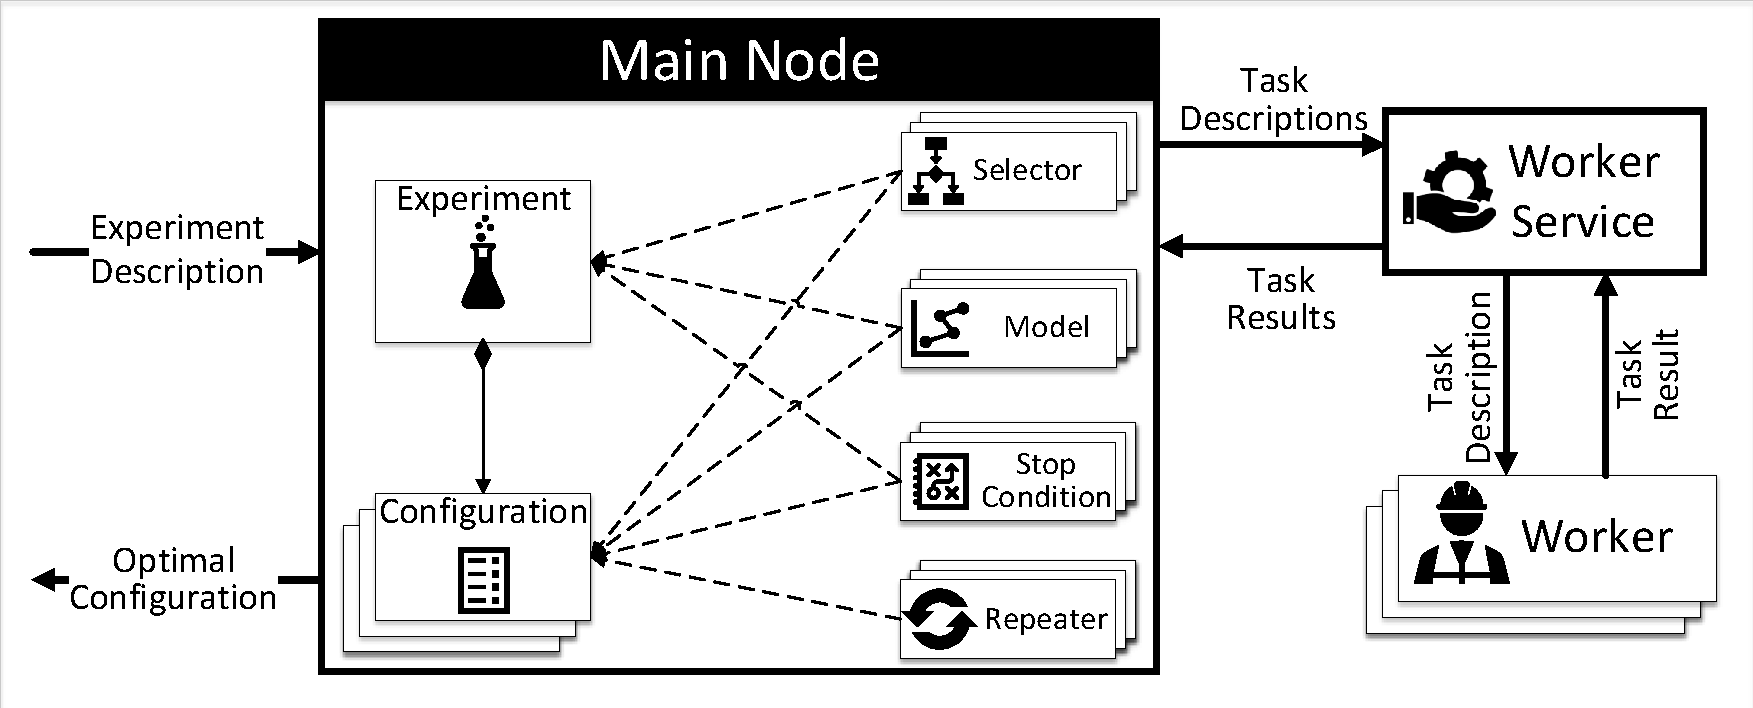
\includegraphics[width=\textwidth]{images/BRISEarch.pdf}
	\caption[The high-level architecture of BRISE]{The high-level architecture of BRISE}
	\label{fig:BRISEarch}
\end{figure}

Figure~\ref{fig:BRISEarch} showns the high-level architecture of BRISE.
Configurable part consists of:
\paragraph{Experiment description} - describes the Experiment, parameters to be tuned, the objective of the experiment, and expected values to detect outliers.
\paragraph{Selector} - Selection Algorithm that is used to get the combination of parameters from the Search Space of all possible parameter combinations. BRISE has two selection algorithms out of the box: Sobol sampling~\cite{sobol99} and the uniform distribution. 
\paragraph{Model} - predicts parameter values. New Model builds after each iteration of measurement of configuration, and if the model predicts a valid result, this configuration goes to be measured in the next iteration. BRISE has several models out of the box.
\paragraph{Stop condition} - the component that analyzes the results of the experiment, validates the result, and makes a decision to stop the experiment or continue. There are many different stop conditions that could work as a combination of criteria.
\paragraph{Repeater} - component of BRISE that decides about the number of measurement for each configuration to get desired accuracy of the results. 
\paragraph{Worker} - contains the process that BRISE needs to tune. Run this process with different configurations and returns the metric of this configuration to use it in the next model build.
All components from the configurable part could be extended by users to achieve their goals.

BRISE has two modes: \textit{Search space exploration} and \textit{Hyperparameter tuning}.
The first mode is used to get information about the search space of hyperparameters. In this mode, there are no predictions because BRISE uses the selector to cover the search space. As a result of using BRISE without predictions, the model component is disabled.

The second mode is used to find the optimized values for hyperparameters. All components of the main node are used in this mode.

The main principle of how BRISE works in both modes is the same, but 
Search space exploration mode has one exception.

The user prepares a target system. Workers call it with specified hyperparameter values and return the results to the BRISE.
After that user describes the experiment description - JSON file that contains all information about hyperparameters, their ranges and default values, result structure, expected ranges for result values, and the max time needed to run one task.

The user input of BRISE is an experiment description that in BRISE is transformed into the experiment object, after that BRISE starts working.

It starts with the measurement of the default configuration. When the default configuration had been measured, the selector gives a set of new configurations to be measured. After measurements, workers return the results to the main node. The repeater checks the result and decides to measure this configuration one more time, or results have needed accuracy. 

On the next step model component tries to build the model and validate it. If a model is valid, then it predicts a new configuration. If the model is not valid, BRISE gets a new configuration from the selector. BRISE sends it to worker service to measure and get the result. If SPL is working in Search space exploration mode, the model build step is skipped, and new configuration is always received from the selector. 

These measurements are being performed until stop condition criteria in stop condition components are met.
